\begin{comment}
\documentclass[12]{report} % Report Mode with font-size 12-pt.
%\documentclass[10]{article} % This sets the mode to article with 10-pt font size.

\usepackage{graphicx} %To facilitate image manipulation, scaling, cropping etc.
\usepackage{rotating}
\usepackage{amsmath}  %Special mathematical formats from Americn Mathmtcl Society.
\usepackage{amssymb}  %Special Symbols from ams. 
\usepackage{algorithm}
\usepackage{algorithmic}
\usepackage{tikz}
\usepackage{verbatim}
\usepackage[T1]{fontenc}
\usepackage{a4}

%\usepackage{algpseudocode}
\addtolength{\textwidth}{8mm}



\begin{document}
\end{comment}
\chapter{Construction of an irregular LDPC codes}\label{chap:"irr"}
\section{Introduction}
In this chapter, first we discuss different parameters that are used to describe an Irregular LDPC code. Then, we give a brief overview about gallager's construction and random construction and list their limitations. Afterwards, as an alternative to previous two methods, we present some methods for the construction of an irregular LDPC code. 

\section{Irregular LDPC code parameters}\label{section:"irrpara"}
From the construction point of view, a LDPC code can be divided into two types: random LDPC code and structured LDPC code. A random LDPC code is constructed using computer search, while structured LDPC code is constructed using algebraic and combinatorial process. Before going to the construction of an Irregular LDPC code, we mention some of the terminologies. An irregular LDPC code is described by edge-perspective degree distribution polynomials for bit and check node. They are defined as:
\begin{equation*}
 \lambda(x)=\sum_d \lambda_dx^{d-1}
\end{equation*}
%
\begin{equation*}
 \rho(x)=\sum_d \rho_dx^{d-1}
\end{equation*}
%
$\lambda(x)$ and $\rho(x)$ are bit and check node edge-perspective degree distribution polynomials, respectively, $\lambda_d$ and $\rho_d$ are fractions of edges connected to a bit and check nodes of degree $d$, respectively.

An irregular LDPC code can also be described using node-perspective degree distribution polynomials for bit and check node as:
\begin{equation*}
 b(x)=\sum_i^{d_b}b_ix^{i}
\end{equation*}
%
\begin{equation*}
 c(x)=\sum_i^{d_c} c_ix^{i}
\end{equation*}
%
Where $b(x)$ and $c(x)$ are bit and check node polynomials, respectively. $b_i$ and $c_i$ are fractions of bit and check nodes of degree $i$, respectively. $d_b$ and $d_c$ are maximum bit and check node degrees, respectively.

Consider a bipartite graph with $n$ bit nodes, $n-k$ check nodes and $E$ edges. Number of edges connected to degree $i$ bit node is:
\begin{equation*}
 \frac{E\lambda_i}{i}
\end{equation*}
%
Since,
\begin{equation*}
 \sum_i \frac{E\lambda_i}{i}=n
\end{equation*}
%
So, total number of edges $E$ is:
\begin{align}
 E&=\frac{n}{\sum_i\frac{\lambda_i}{i}}\nonumber\\
 &=\frac{n}{\int_0^1 \lambda(x)\,\mathrm{d}x}\label{eq1}
\end{align}
%
In the same way, $E$ in terms of $n-k$ is:
\begin{equation}
 E=(n-k) \frac{1}{\int_0^1 \rho(x)\,\mathrm{d}x}\label{eq2}
\end{equation}
%
Comparing Eq.~\eqref{eq1} and \eqref{eq2}:
\begin{equation*}
(n-k)= n \frac{\int_0^1\rho(x)\,\mathrm{d}x}{\int_0^1\lambda(x)\,\mathrm{d}x}
\end{equation*}
%
Assuming parity check matrix to be a full rank, the design rate is given as:
\begin{align}
 R_d&=\frac{k}{n}\nonumber\\
 &=1-\frac{n-k}{n}\nonumber\\
 &=1-\frac{\int_0^1 \rho(x)\,\mathrm{d}x}{\int_0^1 \lambda(x) \,\mathrm{d}x}
\end{align}
%
as shown in \cite{irrldpc}.

\section{An overview of Gallager's and Random construction}
\subsection{Gallager's construction}
This method\cite{Mackay} constructs parity check matrix $H$ with column weight $W_c$ and row weight $W_r$. It first constructs a sub-matrix $H_1$ such that, it contains a single $1$ in each column and $W_r$ 1's in each row. The $i^{th}$ row contains $1$'s in columns $(i-1)W_r + 1$ to $W_r$. Then construct other $W_c-1$ sub matrices by randomly permuting sub-matrix $H_1$. Hence the resultant matrix $H$ is given as:
\begin{align}
 H \overset{\triangle}{=}  \begin{bmatrix}
H_1\\
H_2\\
\vdots\\
H_{W_c}\end{bmatrix} \nonumber
\end{align}

\textbf{Limitations :}
\begin{enumerate}
 \item Do not ensure absence of small cycles
 \item $H$ is not guaranteed to be the full rank, the actual rate $R_a$ may end up very far from the design rate $R_d$
\end{enumerate}

\subsection{Random construction}
The Algorithm is given as:

\begin{algorithm}[H]
\caption{Random construction Algorithm}
\label{rand}
\algsetup{indent=2em}
\begin{algorithmic}
\STATE \textbf{Output:} parity check matrix $H_{n-k \times n}$
\FOR{$i=1$ to $n$}
\STATE choose column $i$ of length $n-k$ such that, it has no more than one $1$-component in common with previously selected columns and all rows weight is less or equal to desired node-perspective degree distribution $c(x)$
\ENDFOR
\end{algorithmic}
\end{algorithm}

\textbf{Limitation :}
For large column weight and code length, computational complexity of this method is very large.

\section{Structured LDPC codes}
An encoding of random codes is quite complex due to lack of code structure. Furthermore, minimum distance of this random code is either very poor or hard to determine\cite{kou}. In proceeding sections, we describe algebraic and combinatorial methods for the construction of a structured irregular code.

\section{Algebraic method}
\subsection{Construction}
In this method the base matrix used is constructed based on the structure of Reed-Solomon Codes\footnote{as described in chap.~\ref{chap:"RS"}}. Thus, resultant irregular code is structured code. Steps involved in the construction of irregular LDPC codes are as follows:
\begin{enumerate}
 \item For the construction of $(\gamma,\rho)$-regular parity check matrix $H_{\gamma q \times \rho q}$ based on Reed-Solomon codes with two information symbols ($m=2$), choose $q^2 \geq N_d,~ q \geq d_c, ~ q \geq d_b$, where $N_d$ is a code length.
 \item Choose $\gamma ~ and ~ \rho$ such that, $\gamma \geq d_b, ~ \rho \geq d_c, ~ \rho q \approxeq N_d ~ and ~ R_d\approxeq (\rho-\gamma)/\rho$
 \item Construct a base matrix $H_{\gamma q \times \rho q}$ and it is given as:
\begin{align}
 H \overset{\triangle}{=}  \begin{bmatrix}
A_{1,1} & A_{1,2} & \cdots & A_{1,\rho}\\
A_{2,1} & A_{2,2} & \cdots & A_{2,\rho}\\
\vdots & \vdots & \vdots & \vdots\\
A_{\gamma,1} & A_{\gamma,2} & \cdots & A_{\gamma,\rho} \end{bmatrix} \nonumber
\end{align}
Where $A_{i,j} ~ (1<i<\gamma ~ and ~ 1<j<\rho)$, is a $q \times q$ permutation matrix
 \item Construct Masking matrix $Z_{\gamma \times \rho}$ such that row (column) weight distribution of $Z$ is equal or approximately equal to $c(x) ~ (b(x))$ of a desired irregular LDPC code. The Masking matrix $Z$ is defined as:
\begin{align}
  Z \overset{\triangle}{=}  \begin{bmatrix}
z_{1,1} & z_{1,2} & \cdots & z_{1,\rho}\\
z_{2,1} & z_{2,2} & \cdots & z_{2,\rho}\\
\vdots & \vdots & \vdots & \vdots\\
z_{\gamma,1} & z_{\gamma,2} & \cdots & z_{\gamma,\rho} \end{bmatrix} \nonumber
\end{align}
 \item Desired irregular LDPC code parity check matrix $H^\prime$ is constructed as follows\cite{geometry}:
\begin{align}
H^\prime&=Z \circledast H \nonumber\\
&=\begin{bmatrix}
z_{1,1}A_{1,1} & z_{1,2}A_{1,2} & \cdots & z_{1,\rho}A_{1,\rho}\\
z_{2,1}A_{2,1} & z_{2,2}A_{2,2} & \cdots & z_{2,\rho}A_{2,\rho}\\
\vdots & \vdots & \vdots & \vdots \\
z_{\gamma,1}A_{\gamma,1} & z_{\gamma,2}A_{\gamma,2} & \cdots & z_{\gamma,\rho}A_{\gamma,\rho} \end{bmatrix} \nonumber
\end{align}

Where, $z_{i,j}A_{i,j}=A_{i,j}$ if $z_{i,j}=1$ and $z_{i,j}A_{i,j}=0_{q \times q}$ if $z_{i,j}=0$.
\end{enumerate}
%
\textbf{Proposition:}
$H^\prime$ has left degree distribution $b(x)$ and right degree distribution $c(x)$
%
\textbf{Proof:}
It follows from construction steps $4$ and $5$.

\subsection{Properties of an Irregular code}
\begin{enumerate}
 \item As RS  based construction ensures that any two rows (columns) of a parity check matrix $H$ have at most $1$-component in common. The previous statement is known as Row-Column (RC) constraint. The RC-constraint implies:
\begin{enumerate}
\item The associated bipartite graph is free of cycles of length 4 and has girth atleat six
\item The minimum distance of  the code is at least $\gamma+1$
\end{enumerate}

As masking operation does not introduce new $1$-component, $H^\prime$ also satisfies the RC-constraint
 \item As $A_{i,j}$'s are permutation matrices, hence they are cycle free. Thus, regardless of girth of bipartite graph of $H$, the girth of bipartite graph of $H^\prime$ is at least equal to that of $Z$.
 \item As size of matrix $Z$ is smaller compared to the size of $H$, it is easier to construct $Z$ using method like progressive edge growth (PEG) with a large girth.
\end{enumerate}

\section{Combinatorial Method}
In this section, we present progressive edge growth (PEG) method for the construction of regular and irregular LDPC code. A bipartite graph can be described using bit nodes, check nodes and set of edges $E$. In this method, edges between bit nodes and check nodes are established in a progressive manner. For given bit node, an edge connects the one of the check node such that girth is maximum. Thus, PEG algorithm has large girth when compared to codes constructed using random methods. Hence, code constructed using PEG algorithm has low error floor in comparison with code constructed using random methods\cite{speg}.

Let us describe bit node degree sequence as follow:
\begin{equation*}
 D_b=\{{d_b}_1,{d_b}_2,\cdots,{d_b}_n\},~ {d_b}_1 \leq {d_b}_2 \leq \cdots \leq {d_b}_n
\end{equation*}
%
Where ${d_b}_i$ presents the degree of $i^{th}$ bit node.

\begin{algorithm}[H]
\caption{Progressive Edge Growth Algorithm\cite{PEG}}
\label{peg}
\algsetup{indent=2em}
\begin{algorithmic}
\STATE \textbf{Input:} sequence $D_b$
\STATE \textbf{Output:} parity check matrix $H$
\STATE initialize all check nodes with degree $0$
\FOR{$i=1$ to $n$}
\FOR{$j=1$ to ${d_b}_i$}
\IF{$j=1$}
\STATE $1.~$find minimum degree check nodes set $C=\{c_1,c_2,\cdots,c_m\},~ 1 \leq m\leq n-k$ such that $deg(c_1)=deg(c_2)=\cdots=deg(c_m)$
\STATE $2.~$choose check node $c_1 \in C$
\STATE $3.~$put an edge between $i^{th}$ bit node and check node $c_1$
\STATE $4.~$increase the degree of $c_1$ by 1
\ELSE
\STATE $1.~$for $i^{th}$ bit node find check nodes set $C=\{c_1,c_2,\cdots,c_m\},~1\leq m\leq n-k$ such that girth is maximum and $deg(c_1) \leq deg(c_2) \leq \cdots \leq deg(c_m)$
\STATE $2.~$put an edge between $i^{th}$ bit node and check node $c_1$ 
\STATE $3.~$increase the degree of $c_1$ by 1
\ENDIF
\ENDFOR
\ENDFOR
\end{algorithmic}
\end{algorithm}
%
Check node degree distribution obtained using Algorithm \ref{peg} is almost uniform. Whenever multiple choices are available to pick check node from set $C$, we can either pick first check node in the set $C$ or pick any check node from set $C$. In algorithm \ref{peg}, we always choose the first member of set $C$.

Now, we show the construction of a $(7,4,3)$ hamming code using algorithm \ref{peg}. In this case, $D_b=\{1,1,1,2,2,2,3\}$. In Figures~\ref{fig:irr1},~\ref{fig:irr2},~\ref{fig:irr3}, dashed blue line represents an edge established in current iteration and red line represents edges that were established in previous iterations.

\begin{sidewaysfigure}[htbp]
\begin{center}
\begin{tikzpicture}[line width=1.0pt,>=stealth,lab/.style={sloped,above,pos=0.9},lab1/.style={sloped,below,pos=0.9}]
\foreach \i in {1,2,3,4,5,6,7}{\draw (0,-2*\i)circle(0.1cm) ++(-0.05,0) node (v\i){};};
\foreach \i in {1,2,3}{\draw (4-0.1,-3-2*\i-0.1)rectangle ++(0.2cm,0.2cm) ++(-0.1cm,-0.1cm) node (c\i){};};
\draw[dashed,color=blue,->] (v1)node[left]{$b_1$} -- (c1)node[right]{$c_1$};
\end{tikzpicture}%\\  
\hspace*{1.0cm}
\begin{tikzpicture}[line width=1.0pt,>=stealth,lab/.style={sloped,above,pos=0.9},lab1/.style={sloped,below,pos=0.9}]
\foreach \i in {1,2,3,4,5,6,7}{\draw (0,-2*\i)circle(0.1cm) ++(-0.05,0) node (v\i){};};
\foreach \i in {1,2,3}{\draw (4-0.1,-3-2*\i-0.1)rectangle ++(0.2cm,0.2cm) ++(-0.1cm,-0.1cm) node (c\i){};};
\draw[color=red,->] (v1)node[left]{$b_1$} -- (c1)node[right]{$c_1$};
\draw[dashed,color=blue,->] (v2)node[left]{$b_2$} -- (c2)node[right]{$c_2$};
\end{tikzpicture}%
\hspace*{1.0cm}
\begin{tikzpicture}[line width=1.0pt,>=stealth,lab/.style={sloped,above,pos=0.9},lab1/.style={sloped,below,pos=0.9}]
\foreach \i in {1,2,3,4,5,6,7}{\draw (0,-2*\i)circle(0.1cm) ++(-0.05,0) node (v\i){};};
\foreach \i in {1,2,3}{\draw (4-0.1,-3-2*\i-0.1)rectangle ++(0.2cm,0.2cm) ++(-0.1cm,-0.1cm) node (c\i){};};
\draw[color=red,->] (v1)node[left]{$b_1$} -- (c1)node[right]{$c_1$};
\draw[color=red,->] (v2)node[left]{$b_2$} -- (c2)node[right]{$c_2$};
\draw[dashed,color=blue,->] (v3)node[left]{$b_3$} -- (c3)node[right]{$c_3$};
\end{tikzpicture}%
\hspace*{1.0cm}
\begin{tikzpicture}[line width=1.0pt,>=stealth,lab/.style={sloped,above,pos=0.9},lab1/.style={sloped,below,pos=0.9}]
\foreach \i in {1,2,3,4,5,6,7}{\draw (0,-2*\i)circle(0.1cm) ++(-0.05,0) node (v\i){};};
\foreach \i in {1,2,3}{\draw (4-0.1,-3-2*\i-0.1)rectangle ++(0.2cm,0.2cm) ++(-0.1cm,-0.1cm) node (c\i){};};
\draw[color=red,->] (v1)node[left]{$b_1$} -- (c1)node[right]{$c_1$};
\draw[color=red,->] (v2)node[left]{$b_2$} -- (c2)node[right]{$c_2$};
\draw[color=red,->] (v3)node[left]{$b_3$} -- (c3)node[right]{$c_3$};
\draw[dashed,color=blue,->] (v4)node[left]{$b_4$} -- (c1);
\end{tikzpicture}%
\end{center}
\caption[PEG algorithm: $i=1~and~j=1,i=2~and~j=1,i=3~and~j=1,i=4~and~j=1$]%
{\label{fig:irr1}In the beginning, $i=1,j=1$, all check nodes have degree $0$. Thus, set $C$ is $\{deg(c_1)=0,deg(c_2)=0,deg(c_3)=0\}$. Hence, this algorithm connects bit node $b_1$ to the check node $c_1$ and it is shown in the left most figure. Now degree of check node $c_1$ is $1$. For $i=2,j=1$, set $C$ is $\{deg(c_2)=0,deg(c_3)=0,deg(c_1)=1\}$. So, according to algorithm bit node $b_2$ is connected with check node $c_2$ and it is shown in the second figure. For $i=3,j=1$, set $C$ is $\{deg(c_3)=0,deg(c_2)=1,deg(c_1)=1\}$. So, according to algorithm bit node $b_3$ is connected with check node $c_3$ and it is shown in the third figure. For $i=4,j=1$, set $C$ is $\{deg(c_1)=1,deg(c_2)=1,deg(c_3)=1\}$. So, according to algorithm bit node $b_4$ is connected with check node $c_1$ and it is shown in right most figure.}
\end{sidewaysfigure}

\begin{sidewaysfigure}[htbp]
\begin{center}
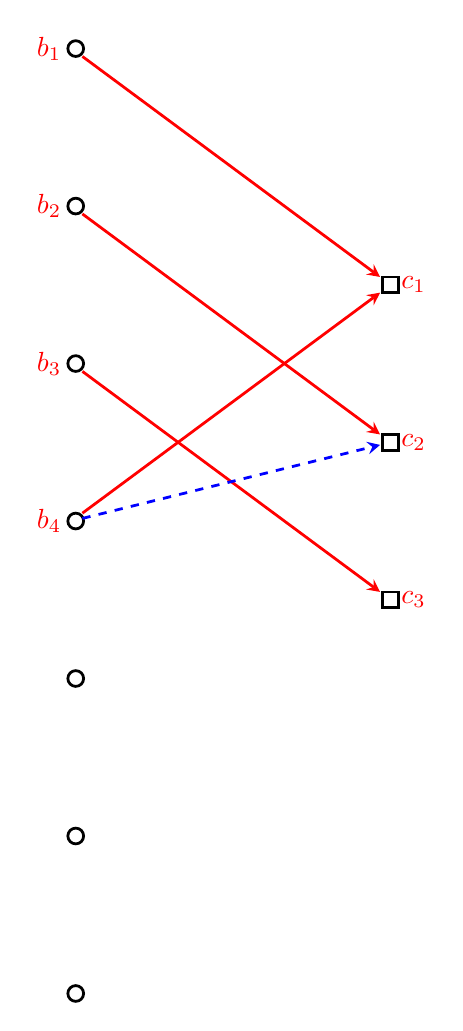
\begin{tikzpicture}[line width=1.0pt,>=stealth,lab/.style={sloped,above,pos=0.9},lab1/.style={sloped,below,pos=0.9}]
\foreach \i in {1,2,3,4,5,6,7}{\draw (0,-2*\i)circle(0.1cm) ++(-0.05,0) node (v\i){};};
\foreach \i in {1,2,3}{\draw (4-0.1,-3-2*\i-0.1)rectangle ++(0.2cm,0.2cm) ++(-0.1cm,-0.1cm) node (c\i){};};
\draw[color=red,->] (v1)node[left]{$b_1$} -- (c1)node[right]{$c_1$};
\draw[color=red,->] (v2)node[left]{$b_2$} -- (c2)node[right]{$c_2$};
\draw[color=red,->] (v3)node[left]{$b_3$} -- (c3)node[right]{$c_3$};
\draw[color=red,->] (v4)node[left]{$b_4$} -- (c1);
\draw[dashed,color=blue,->] (v4) -- (c2);
\end{tikzpicture}%
\hspace*{1.0cm}
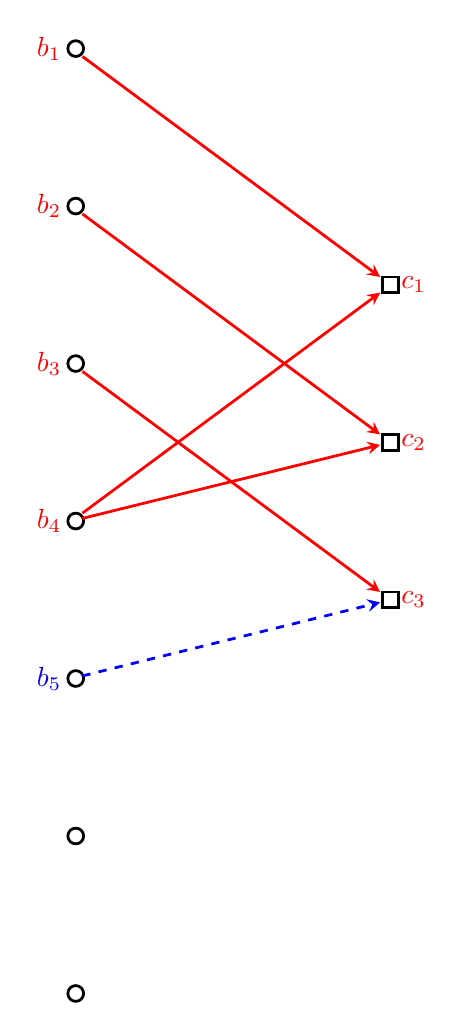
\begin{tikzpicture}[line width=1.0pt,>=stealth,lab/.style={sloped,above,pos=0.9},lab1/.style={sloped,below,pos=0.9}]
\foreach \i in {1,2,3,4,5,6,7}{\draw (0,-2*\i)circle(0.1cm) ++(-0.05,0) node (v\i){};};
\foreach \i in {1,2,3}{\draw (4-0.1,-3-2*\i-0.1)rectangle ++(0.2cm,0.2cm) ++(-0.1cm,-0.1cm) node (c\i){};};
\draw[color=red,->] (v1)node[left]{$b_1$} -- (c1)node[right]{$c_1$};
\draw[color=red,->] (v2)node[left]{$b_2$} -- (c2)node[right]{$c_2$};
\draw[color=red,->] (v3)node[left]{$b_3$} -- (c3)node[right]{$c_3$};
\draw[color=red,->] (v4)node[left]{$b_4$} -- (c1);
\draw[color=red,->] (v4) -- (c2);
\draw[dashed,color=blue,->] (v5)node[left]{$b_5$} -- (c3);
\end{tikzpicture}%
\hspace*{1.0cm}
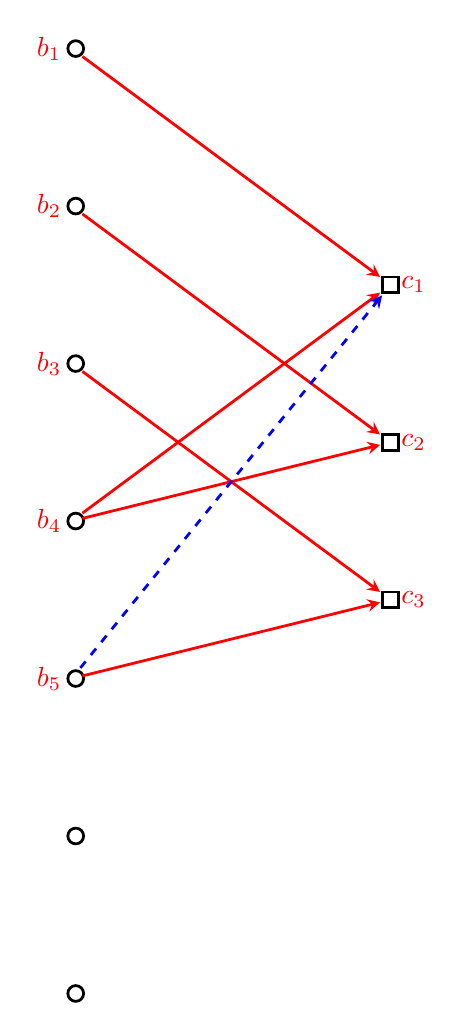
\begin{tikzpicture}[line width=1.0pt,>=stealth,lab/.style={sloped,above,pos=0.9},lab1/.style={sloped,below,pos=0.9}]
\foreach \i in {1,2,3,4,5,6,7}{\draw (0,-2*\i)circle(0.1cm) ++(-0.05,0) node (v\i){};};
\foreach \i in {1,2,3}{\draw (4-0.1,-3-2*\i-0.1)rectangle ++(0.2cm,0.2cm) ++(-0.1cm,-0.1cm) node (c\i){};};
\draw[color=red,->] (v1)node[left]{$b_1$} -- (c1)node[right]{$c_1$};
\draw[color=red,->] (v2)node[left]{$b_2$} -- (c2)node[right]{$c_2$};
\draw[color=red,->] (v3)node[left]{$b_3$} -- (c3)node[right]{$c_3$};
\draw[color=red,->] (v4)node[left]{$b_4$} -- (c1);
\draw[color=red,->] (v4) -- (c2);
\draw[color=red,->] (v5)node[left]{$b_5$} -- (c3);
\draw[dashed,color=blue,->] (v5) -- (c1);
\end{tikzpicture}%
\hspace*{1.0cm}
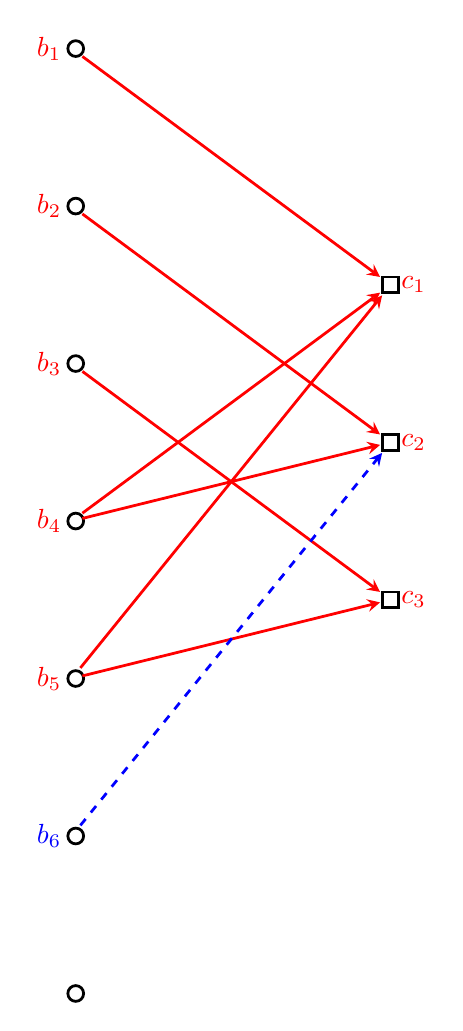
\begin{tikzpicture}[line width=1.0pt,>=stealth,lab/.style={sloped,above,pos=0.9},lab1/.style={sloped,below,pos=0.9}]
\foreach \i in {1,2,3,4,5,6,7}{\draw (0,-2*\i)circle(0.1cm) ++(-0.05,0) node (v\i){};};
\foreach \i in {1,2,3}{\draw (4-0.1,-3-2*\i-0.1)rectangle ++(0.2cm,0.2cm) ++(-0.1cm,-0.1cm) node (c\i){};};
\draw[color=red,->] (v1)node[left]{$b_1$} -- (c1)node[right]{$c_1$};
\draw[color=red,->] (v2)node[left]{$b_2$} -- (c2)node[right]{$c_2$};
\draw[color=red,->] (v3)node[left]{$b_3$} -- (c3)node[right]{$c_3$};
\draw[color=red,->] (v4)node[left]{$b_4$} -- (c1);
\draw[color=red,->] (v4) -- (c2);
\draw[color=red,->] (v5)node[left]{$b_5$} -- (c1);
\draw[color=red,->] (v5) -- (c3);
\draw[dashed,color=blue,->] (v6)node[left]{$b_6$} -- (c2);
\end{tikzpicture}%
\end{center}
\caption[PEG algorithm: $i=4~and~j=2,i=5~and~j=1,i=5~and~j=2,i=6~and~j=1$]%
{\label{fig:irr2}For $i=4,j=2$, set $C$ according to maximum girth and minimum degree of check node $\{c_2,c_3,c_1\}$. So, according to algorithm bit node $b_4$ is connected with check node $c_2$ and it is shown in left most figure. For $i=5,j=1$, set $C$ is $\{deg(c_3)=1,deg(c_2)=2,deg(c_1)=2\}$. So, according to algorithm bit node $b_5$ is connected with check node $c_3$ and it is shown in the second figure. For $i=5,j=2$, set $C$ according to maximum girth and minimum degree of check node $\{c_1,c_2,c_3\}$. So, according to algorithm bit node $b_5$ is connected with check node $c_1$ and it is shown in the third figure. For $i=6,j=1$, set $C$ is $\{deg(c_2)=2,deg(c_3)=2,deg(c_1)=3\}$. So, according to algorithm bit node $b_6$ is connected with check node $c_2$ and it is shown in right most figure.}
\end{sidewaysfigure}

\begin{sidewaysfigure}[htbp]
\begin{center}
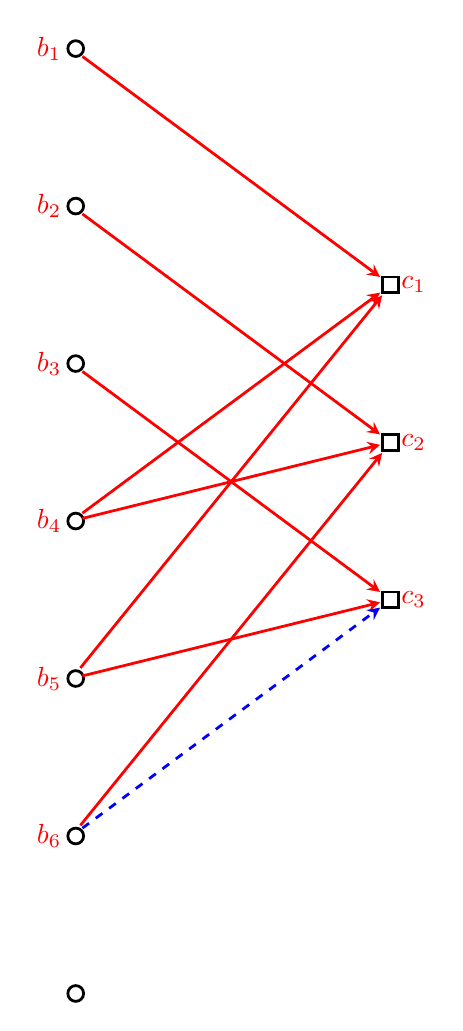
\begin{tikzpicture}[line width=1.0pt,>=stealth,lab/.style={sloped,above,pos=0.9},lab1/.style={sloped,below,pos=0.9}]
\foreach \i in {1,2,3,4,5,6,7}{\draw (0,-2*\i)circle(0.1cm) ++(-0.05,0) node (v\i){};};
\foreach \i in {1,2,3}{\draw (4-0.1,-3-2*\i-0.1)rectangle ++(0.2cm,0.2cm) ++(-0.1cm,-0.1cm) node (c\i){};};
\draw[color=red,->] (v1)node[left]{$b_1$} -- (c1)node[right]{$c_1$};
\draw[color=red,->] (v2)node[left]{$b_2$} -- (c2)node[right]{$c_2$};
\draw[color=red,->] (v3)node[left]{$b_3$} -- (c3)node[right]{$c_3$};
\draw[color=red,->] (v4)node[left]{$b_4$} -- (c1);
\draw[color=red,->] (v4) -- (c2);
\draw[color=red,->] (v5)node[left]{$b_5$} -- (c1);
\draw[color=red,->] (v5) -- (c3);
\draw[color=red,->] (v6)node[left]{$b_6$} -- (c2);
\draw[dashed,color=blue,->] (v6) -- (c3);
\end{tikzpicture}%
\hspace*{1.0cm}
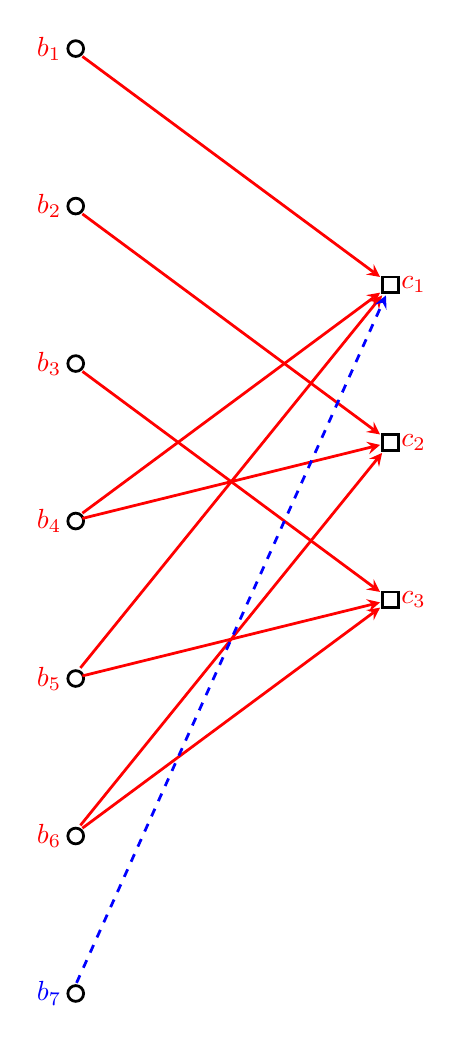
\begin{tikzpicture}[line width=1.0pt,>=stealth,lab/.style={sloped,above,pos=0.9},lab1/.style={sloped,below,pos=0.9}]
\foreach \i in {1,2,3,4,5,6,7}{\draw (0,-2*\i)circle(0.1cm) ++(-0.05,0) node (v\i){};};
\foreach \i in {1,2,3}{\draw (4-0.1,-3-2*\i-0.1)rectangle ++(0.2cm,0.2cm) ++(-0.1cm,-0.1cm) node (c\i){};};
\draw[color=red,->] (v1)node[left]{$b_1$} -- (c1)node[right]{$c_1$};
\draw[color=red,->] (v2)node[left]{$b_2$} -- (c2)node[right]{$c_2$};
\draw[color=red,->] (v3)node[left]{$b_3$} -- (c3)node[right]{$c_3$};
\draw[color=red,->] (v4)node[left]{$b_4$} -- (c1);
\draw[color=red,->] (v4) -- (c2);
\draw[color=red,->] (v5)node[left]{$b_5$} -- (c1);
\draw[color=red,->] (v5) -- (c3);
\draw[color=red,->] (v6)node[left]{$b_6$} -- (c2);
\draw[color=red,->] (v6) -- (c3);
\draw[dashed,color=blue,->] (v7)node[left]{$b_7$} -- (c1);
\end{tikzpicture}%
\hspace*{1.0cm}
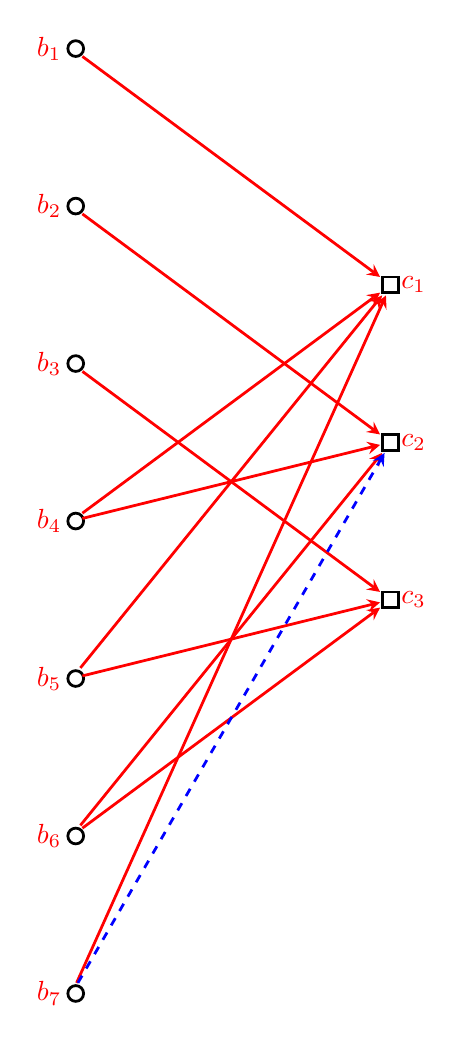
\begin{tikzpicture}[line width=1.0pt,>=stealth,lab/.style={sloped,above,pos=0.9},lab1/.style={sloped,below,pos=0.9}]
\foreach \i in {1,2,3,4,5,6,7}{\draw (0,-2*\i)circle(0.1cm) ++(-0.05,0) node (v\i){};};
\foreach \i in {1,2,3}{\draw (4-0.1,-3-2*\i-0.1)rectangle ++(0.2cm,0.2cm) ++(-0.1cm,-0.1cm) node (c\i){};};
\draw[color=red,->] (v1)node[left]{$b_1$} -- (c1)node[right]{$c_1$};
\draw[color=red,->] (v2)node[left]{$b_2$} -- (c2)node[right]{$c_2$};
\draw[color=red,->] (v3)node[left]{$b_3$} -- (c3)node[right]{$c_3$};
\draw[color=red,->] (v4)node[left]{$b_4$} -- (c1);
\draw[color=red,->] (v4) -- (c2);
\draw[color=red,->] (v5)node[left]{$b_5$} -- (c1);
\draw[color=red,->] (v5) -- (c3);
\draw[color=red,->] (v6)node[left]{$b_6$} -- (c2);
\draw[color=red,->] (v6) -- (c3);
\draw[color=red,->] (v7)node[left]{$b_7$} -- (c1);
\draw[dashed,color=blue,->] (v7) -- (c2);
\end{tikzpicture}%
\hspace*{1.0cm}
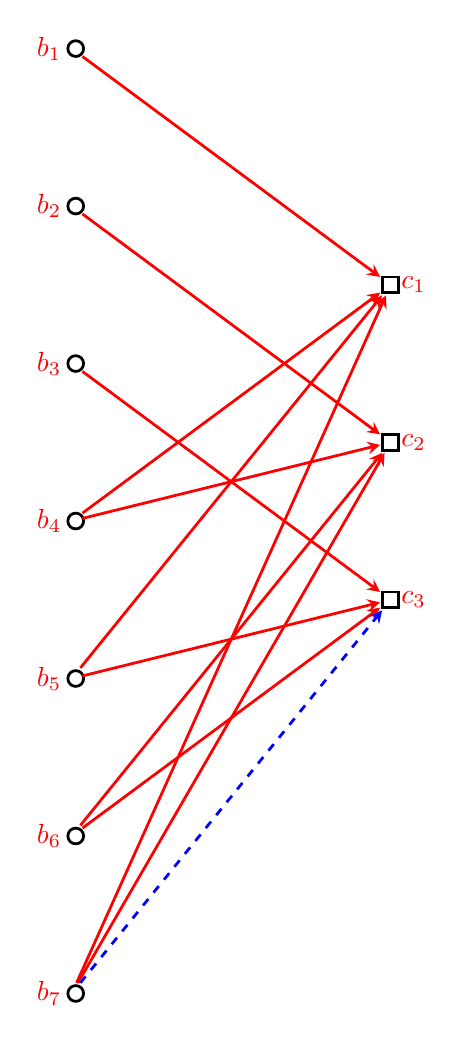
\begin{tikzpicture}[line width=1.0pt,>=stealth,lab/.style={sloped,above,pos=0.9},lab1/.style={sloped,below,pos=0.9}]
\foreach \i in {1,2,3,4,5,6,7}{\draw (0,-2*\i)circle(0.1cm) ++(-0.05,0) node (v\i){};};
\foreach \i in {1,2,3}{\draw (4-0.1,-3-2*\i-0.1)rectangle ++(0.2cm,0.2cm) ++(-0.1cm,-0.1cm) node (c\i){};};
\draw[color=red,->] (v1)node[left]{$b_1$} -- (c1)node[right]{$c_1$};
\draw[color=red,->] (v2)node[left]{$b_2$} -- (c2)node[right]{$c_2$};
\draw[color=red,->] (v3)node[left]{$b_3$} -- (c3)node[right]{$c_3$};
\draw[color=red,->] (v4)node[left]{$b_4$} -- (c1);
\draw[color=red,->] (v4) -- (c2);
\draw[color=red,->] (v5)node[left]{$b_5$} -- (c1);
\draw[color=red,->] (v5) -- (c3);
\draw[color=red,->] (v6)node[left]{$b_6$} -- (c2);
\draw[color=red,->] (v6) -- (c3);
\draw[color=red,->] (v7)node[left]{$b_7$} -- (c1);
\draw[color=red,->] (v7) -- (c2);
\draw[dashed,color=blue,->] (v7) -- (c3);
\end{tikzpicture}%
\end{center}
\caption[PEG algorithm: $i=6~and~j=2,i=7~and~j=1,i=7~and~j=2,i=7~and~j=3$]%
{\label{fig:irr3}For $i=6,j=2$, set $C$ according to maximum girth and minimum degree of check node is $\{c_3,c_1,c_2\}$. So, according to algorithm bit node $b_6$ is connected with check node $c_3$ and it is shown in left most figure. For $i=7,j=1$, set $C$ is $\{deg(c_1)=3,deg(c_2)=3,deg(c_3)=3\}$. So, according to algorithm bit node $b_7$ is connected with check node $c_1$ and it is shown in the second figure. For $i=7,j=2$, set $C$ according to maximum girth and minimum degree of check node is $\{c_2,c_3,c_1\}$. So, according to algorithm bit node $b_7$ is connected with check node $c_2$ and it is shown in the third figure. For $i=7,j=3$, set $C$ according to maximum girth and minimum degree of check node is $\{c_3,c_2,c_1\}$. So, according to algorithm bit node $b_7$ is connected with check node $c_3$ and it is shown in right most figure.}
\end{sidewaysfigure}

The resultant parity check matrix $H$ is given as:
\begin{align}
  H =  \begin{bmatrix}
1 & 0 & 0 & 1 & 1 & 0 &1\\
0 & 1 & 0 & 1 & 0 & 1 &1\\
0 & 0 & 1 & 0 & 1 & 1 &1\\ \end{bmatrix} \nonumber
\end{align}

In this chapter we have shown the construction of an irregular LDPC codes using An algebraic method and the PEG algorithm. In next chapter, we show the encoding procedure.
\begin{comment}
\begin{thebibliography}{99}

\bibitem{irrldpc} Thomas J.~Richardson, M.~Amin Shokrollahi, Member, IEEE, and Rudiger L.~Urbanke. ``Design of Capacity-Approaching Irregular Low-Density Parity-Check Codes'', IEEE Transactions On Information Theory, VOL. $47$, NO.$2$, FEBRUARY $2001$.
\bibitem{Mackay} David J.~c.~Mackay. ``Good Error-Correcting Codes Based on Very Sparse Matrices'', IEEE Transactions On Information Theory, VOL. $45$, NO.$2$, MARCH $1999$.
\bibitem{kou} Y.~Kou, S.~Lin, and M.~Fossorier, ``Low density parity check codes based on finite geometries: A rediscovery and new results'', IEEE Transactions On Information Theory, VOL. $47$, NO.$7$, pp.~$2711-2736$, Nov.~ $2001$.
\bibitem{geometry} Jun Xu, Member, IEEE, Lei Chen, Ivana Djurdjevic, Shu Lin, Life Fellow, IEEE, and Khaled Abdel-Ghaggar, Member, IEEE. ``Construction of Regular and Irregular LDPC codes: Geometry Decomposition and Masking'', IEEE Transactions On Information Theory, VOL. $53$, NO.$1$, January $2007$.
\bibitem{speg} Lam Pham Sy, Valentin Savin, David Declercq, Nghia Pham, Eutelsat, Paris, France, CEA-LETI, MINATEC campus, Grenoble, France, ENSEA, Cergy-Pontoise, France. ``Scheduled-PEG construction of LDPC codes for Upper-Layer FEC''.
\bibitem{PEG} Xiao-Yu Hu, Member, IEEE, Evangelos Eleftheriou, Fellow, IEEE, and Dieter M. ~ Arnold, Member, IEEE. ``Regular and Irregular Progressive Edge-Growth Tanner Graphs'', IEEE Transactions On Information Theory, VOL. $51$, NO.$1$, January $2005$.

\end{thebibliography}


\end{document}
\end{comment}
